\documentclass[11pt]{article}
\usepackage[T1]{fontenc}
\usepackage[latin1]{inputenc}
\usepackage{enumerate}
\usepackage{setspace}
\usepackage{amsmath,amssymb,amsthm}
\usepackage{graphicx}
\usepackage{bbm}
\usepackage[round]{natbib}
\usepackage[nohead]{geometry}
\usepackage[bottom]{footmisc}
\usepackage{indentfirst}
\usepackage{endnotes}
\usepackage{graphicx}%
\usepackage{eurosym}
\usepackage{array}
\usepackage{booktabs}
\usepackage{caption}
\usepackage{subcaption}
\usepackage{rotating}
% \usepackage[hidelinks]{hyperref}
\usepackage{floatrow} %[capposition=top]
\floatsetup{footposition=bottom,capposition=top}
\renewcommand{\labelitemi}{--}
\renewcommand{\labelitemii}{$\bullet$}
\bibliographystyle{chicago}
% \geometry{left=1in,right=1in,top=1.00in,bottom=1.0in}
\let\olditemize\itemize
\renewcommand{\itemize}{
  \olditemize
  \setlength{\itemsep}{-1pt}
}

\begin{document}

\title{French grocery stores\ \\ \ \\(Very preliminary)}
\author{Etienne Chamayou\thanks{e-mail:
\textit{etienne.chamayou@ensae.fr}}\medskip\\{\normalsize CREST and Department of Economics, Ecole Polytechnique }}
\maketitle

\sloppy%

\onehalfspacing

\textbf{Abstract:}

This note provides an overview of French grocery stores in 2014. All the analysis relies on data provided by LSA on hypermarkets, supermarkets, hard discount stores and "drive-through".

\strut

\textbf{Keywords:} 

\strut

\textbf{JEL Classification Numbers:} XXX

\pagebreak%
\doublespacing

\section{Introduction}

Data provided by LSA include17,254 French grocery stores. LSA provide three columns regarding the activity of stores over time: an opening date, a closing date and a reopenening date. Stores can thus be considered closed when they have a closing date but no reopening date. According to LSA data, beginning 2014, there were 15,086 hypermarkets, supermarkets, hard discount and "drive-through" stores operating in France. 

\section{Overview of store population by type}

\subsection{Surface by type}

Descriptive statistics on surface by type show that grocery stores with a surface between 400 and 2500 $m^2$ are categorized as supermarkets, while those with a surface exceeding 2500 $m^2$ are categorized as hypermarkets. The type "Magasins Populaires" is attributed to stores with a significant surface dedicated to non food products (most of them belong to the same retail chain as will be shown later).

\begin{table}[H]
\caption{Surface in $m^2$ by type of store}
\small
\begin{tabular}{lrrrrrrr}
\toprule
{} &       \#Tot &      \#Null &        Avg &        Med &        Min &        Max &        Cum \\
\midrule
Supermarkets         &       5644 &        nan &       1277 &       1200 &        400 &       2499 &    7204724 \\
Hard discount        &       4556 &        nan &        767 &        770 &        100 &       2400 &    3496484 \\
Drive in             &       2055 &       1807 &       1390 &       1500 &         10 &       3900 &     344776 \\
Hypermarkets         &       2013 &        nan &       5414 &       4115 &       2500 &      24000 &   10899121 \\
Drive                &        438 &        nan &       1803 &       1800 &        100 &       7500 &     789814 \\
"Magasins populaires &        380 &        nan &       1514 &       1422 &        210 &       5154 &     575345 \\
\bottomrule
\multicolumn{8}{l}{The "\#Null" colum indicates the number of missing values.} \\
\end{tabular}
\end{table}

\subsection{Number of checkouts by type}

\begin{table}[H]
\caption{Number of checkouts by type of store}
\small
\begin{tabular}{lrrrrrrr}
\toprule
{} &       \#Tot &      \#Null &        Avg &        Med &        Min &        Max &        Cum \\
\midrule
Supermarkets         &       5644 &        nan &          7 &          6 &          1 &         25 &      37751 \\
Hard discount        &       4556 &          1 &          4 &          4 &          1 &         42 &      19671 \\
Drive in             &       2055 &        523 &          2 &          1 &          1 &         17 &       3533 \\
Hypermarkets         &       2013 &          2 &         23 &         19 &          2 &        358 &      46858 \\
Drive                &        438 &        nan &          7 &          7 &          1 &         85 &       3173 \\
"Magasins populaires &        380 &        nan &         10 &          8 &          1 &         34 &       3855 \\
\bottomrule
\end{tabular}
\end{table}

\subsection{Size of Parking by type}

\begin{table}[H]
\caption{Size of parking by type of store}
\small
\begin{tabular}{lrrrrrrr}
\toprule
{} &       \#Tot &  \#Null &        Avg &        Med &        Min &        Max &        Cum \\
\midrule
Supermarkets         &       5644 &   1308 &        135 &        120 &          2 &       2577 &     584036 \\
Hard discount        &       4556 &   3037 &         87 &         72 &          3 &       1200 &     132500 \\
Drive in             &       2055 &   2055 &        nan &        nan &        nan &        nan &        nan \\
Hypermarkets         &       2013 &     79 &        763 &        500 &         40 &       7660 &    1476596 \\
Drive                &        438 &    436 &         39 &         39 &         38 &         40 &         78 \\
"Magasins populaires &        380 &    308 &        254 &        100 &         15 &       3500 &      18320 \\
\bottomrule
\end{tabular}
\end{table}

\subsection{Number of gas pumps}

\begin{table}[H]
\caption{Number of gas pumps by type of store}
\small
\begin{tabular}{lrrrrrrr}
\toprule
{} &       \#Tot &  \#Null &        Avg &        Med &        Min &        Max &        Cum \\
\midrule
Supermarkets         &       5644 &   2732 &          4 &          4 &          0 &         16 &      11564 \\
Hard discount        &       4556 &   4425 &          4 &          4 &          1 &         23 &        519 \\
Drive in             &       2055 &     17 &          3 &          2 &          1 &         28 &       6801 \\
Hypermarkets         &       2013 &    226 &          8 &          7 &          1 &         26 &      13958 \\
Drive                &        438 &      1 &          9 &          8 &          2 &         35 &       3924 \\
"Magasins populaires &        380 &    378 &          4 &          4 &          4 &          4 &          8 \\
\bottomrule
\end{tabular}
\end{table}

\section{Stores and surface by group and chain}

This section focuses on hypermarkets, supermarkets and hard discount stores (exclude?). "Drive-through" are thus left aside.

\subsection{Stores and surface by group}

The following table shows the number of hypermarkets, supermarkets and hard discount stores operated by the main grocery store groups in France. 

\begin{table}[H]
\footnotesize
\setlength{\tabcolsep}{2pt}
\begin{tabular}{lrrrrrrrrrr}
\toprule
{} &       \#Tot &       \#Hyp &       \#Sup &       \#Dis &        \#MP &     Avg S. &     Med S. &     Min S. &     Max S. &     Cum S. \\
\midrule
CARREFOUR      &       2588 &        381 &       1387 &        820 &          0 &       1885 &        969 &        215 &      24000 &    4878697 \\
CASINO         &       2185 &        175 &        947 &        687 &        376 &       1414 &        900 &        100 &      17112 &    3089516 \\
MOUSQUETAIRES  &       2140 &        348 &       1464 &        328 &          0 &       1672 &       1582 &        100 &       6710 &    3578168 \\
LIDL           &       1522 &          0 &          0 &       1522 &          0 &        824 &        830 &        250 &       1900 &    1253932 \\
SYSTEME U      &       1099 &        344 &        755 &          0 &          0 &       2138 &       2000 &        400 &      11750 &    2349901 \\
ALDI           &        917 &          0 &          0 &        917 &          0 &        698 &        720 &        281 &       1300 &     640460 \\
LECLERC        &        652 &        527 &        125 &          0 &          0 &       4627 &       4390 &        400 &      15600 &    3016627 \\
AUCHAN         &        574 &        161 &        413 &          0 &          0 &       3521 &       1639 &        400 &      19700 &    2021138 \\
LOUIS DELHAIZE &        203 &         70 &        133 &          0 &          0 &       3976 &       1950 &        450 &      15500 &     807116 \\
DIAPAR         &        116 &          0 &        116 &          0 &          0 &        533 &        400 &        400 &       1200 &      61823 \\
COLRUYT        &        110 &          0 &        110 &          0 &          0 &        837 &        900 &        400 &       1700 &      92023 \\
OTHER          &        487 &          7 &        194 &        282 &          4 &        793 &        680 &        134 &       8700 &     386273 \\
\bottomrule
\end{tabular}
\end{table}

\subsection{Stores and surface by group and chain}

Except for Aldi and Lidl, stores are subdivided in retail chains based on criteria such as the size or the location (city center, suburb, countryside etc.).

\begin{table}[H]
\footnotesize
\setlength{\tabcolsep}{2pt}
\begin{tabular}{lrrrrrrrrrr}
\toprule
CARREFOUR &       \#Tot &       \#Hyp &       \#Sup &       \#Dis &        \#MP &     Avg S. &     Med S. &     Min S. &     Max S. &     Cum S. \\
\midrule
DIA \%              &        819 &          0 &          0 &        819 &          0 &        720 &        782 &        215 &       1280 &     589710 \\
CARREFOUR MARKET   &        809 &        115 &        694 &          0 &          0 &       1891 &       1800 &        654 &       5600 &    1530023 \\
CARREFOUR CONTACT  &        405 &          0 &        405 &          0 &          0 &        681 &        670 &        400 &       1800 &     275872 \\
CARREFOUR          &        228 &        228 &          0 &          0 &          0 &       9223 &       8820 &       2500 &      24000 &    2102841 \\
CARREFOUR CITY     &        124 &          0 &        124 &          0 &          0 &        504 &        450 &        400 &        800 &      62472 \\
MARKET             &        121 &         37 &         84 &          0 &          0 &       2204 &       2200 &        722 &       4500 &     266736 \\
SHOPI              &         34 &          0 &         34 &          0 &          0 &        573 &        500 &        400 &        870 &      19494 \\
CARREFOUR EXPRESS  &         21 &          0 &         21 &          0 &          0 &        475 &        460 &        400 &        750 &       9981 \\
CHAMPION           &          7 &          0 &          7 &          0 &          0 &       1272 &       1200 &        600 &       1860 &       8905 \\
PROXI              &          7 &          0 &          7 &          0 &          0 &        482 &        450 &        400 &        821 &       3376 \\
CARREFOUR MONTAGNE &          4 &          0 &          4 &          0 &          0 &        500 &        500 &        450 &        550 &       2000 \\
PROXI SUPER        &          4 &          0 &          4 &          0 &          0 &        520 &        550 &        430 &        550 &       2080 \\
8 A HUIT           &          3 &          0 &          3 &          0 &          0 &        407 &        400 &        400 &        420 &       1220 \\
ED                 &          1 &          0 &          0 &          1 &          0 &        487 &        487 &        487 &        487 &        487 \\
HYPER CHAMPION     &          1 &          1 &          0 &          0 &          0 &       3500 &       3500 &       3500 &       3500 &       3500 \\
\bottomrule
\end{tabular}
\end{table}

\begin{table}[H]
\footnotesize
\setlength{\tabcolsep}{2pt}
\begin{tabular}{lrrrrrrrrrr}
\toprule
CASINO &       \#Tot &       \#Hyp &       \#Sup &       \#Dis &        \#MP &     Avg S. &     Med S. &     Min S. &     Max S. &     Cum S. \\
\midrule
LEADER PRICE     &        676 &          0 &          1 &        675 &          0 &        891 &        900 &        100 &       2400 &     602195 \\
FRANPRIX         &        448 &          0 &        448 &          0 &          0 &        608 &        500 &        400 &       2400 &     272411 \\
CASINO           &        352 &         16 &        336 &          0 &          0 &       1511 &       1500 &        400 &       3000 &     531832 \\
MONOPRIX         &        301 &          0 &          0 &          0 &        301 &       1792 &       1653 &        297 &       5154 &     539317 \\
SPAR             &        123 &          0 &        123 &          0 &          0 &        562 &        550 &        400 &       1200 &      69135 \\
GEANT CASINO     &        112 &        112 &          0 &          0 &          0 &       7433 &       7396 &       3000 &      17112 &     832482 \\
MONOP'           &         75 &          0 &          0 &          0 &         75 &        356 &        300 &        210 &       1000 &      26728 \\
HYPER CASINO     &         45 &         38 &          7 &          0 &          0 &       3136 &       2800 &       2160 &       5950 &     141138 \\
CASINO SHOPPING  &         11 &          0 &         11 &          0 &          0 &        515 &        500 &        400 &        698 &       5662 \\
JUMBO SCORE      &          9 &          9 &          0 &          0 &          0 &       5103 &       5700 &       2997 &       6000 &      45927 \\
LEADER EXPRESS   &          9 &          0 &          0 &          9 &          0 &        406 &        400 &        260 &        513 &       3658 \\
SCORE            &          9 &          0 &          9 &          0 &          0 &       1132 &        995 &        720 &       1800 &      10186 \\
SPAR SUPERMARCHE &          9 &          0 &          9 &          0 &          0 &        572 &        535 &        400 &       1000 &       5151 \\
LEADER MARKET    &          3 &          0 &          0 &          3 &          0 &        701 &        705 &        670 &        729 &       2104 \\
PETIT CASINO     &          3 &          0 &          3 &          0 &          0 &        530 &        540 &        450 &        600 &       1590 \\
\bottomrule
\end{tabular}
\end{table}

\begin{table}[H]
\footnotesize
\setlength{\tabcolsep}{2pt}
\begin{tabular}{lrrrrrrrrrr}
\toprule
MOUSQUETAIRES &       \#Tot &       \#Hyp &       \#Sup &       \#Dis &        \#MP &     Avg S. &     Med S. &     Min S. &     Max S. &     Cum S. \\
\midrule
INTERMARCHE SUPER        &       1362 &        252 &       1110 &          0 &          0 &       1947 &       1950 &        499 &       4100 &    2651505 \\
NETTO                    &        328 &          0 &          0 &        328 &          0 &        746 &        704 &        100 &       1780 &     244709 \\
INTERMARCHE CONTACT      &        312 &          0 &        312 &          0 &          0 &        804 &        800 &        400 &       1500 &     250860 \\
INTERMARCHE HYPER        &         96 &         96 &          0 &          0 &          0 &       4119 &       4000 &       2800 &       6710 &     395413 \\
INTERMARCHE EXPRESS      &         37 &          0 &         37 &          0 &          0 &        878 &        928 &        400 &       1340 &      32473 \\
RELAIS DES MOUSQUETAIRES &          3 &          0 &          3 &          0 &          0 &        533 &        500 &        400 &        700 &       1600 \\
ECOMARCHE                &          2 &          0 &          2 &          0 &          0 &        804 &        804 &        620 &        988 &       1608 \\
\bottomrule
\end{tabular}
\end{table}

\begin{table}[H]
\footnotesize
\setlength{\tabcolsep}{2pt}
\begin{tabular}{lrrrrrrrrrr}
\toprule
SYSTEME U &       \#Tot &       \#Hyp &       \#Sup &       \#Dis &        \#MP &     Avg S. &     Med S. &     Min S. &     Max S. &     Cum S. \\
\midrule
SUPER U   &        751 &        273 &        478 &          0 &          0 &       2311 &       2245 &        400 &       5200 &    1735315 \\
U EXPRESS &        236 &          1 &        235 &          0 &          0 &        862 &        802 &        400 &       2854 &     203443 \\
HYPER U   &         70 &         70 &          0 &          0 &          0 &       5543 &       5250 &       3003 &      11750 &     388003 \\
UTILE     &         32 &          0 &         32 &          0 &          0 &        486 &        455 &        400 &        700 &      15556 \\
MARCHE U  &         10 &          0 &         10 &          0 &          0 &        758 &        765 &        450 &       1000 &       7584 \\
\bottomrule
\end{tabular}
\end{table}

\begin{table}[H]
\footnotesize
\setlength{\tabcolsep}{2pt}
\begin{tabular}{lrrrrrrrrrr}
\toprule
LECLERC &       \#Tot &       \#Hyp &       \#Sup &       \#Dis &        \#MP &     Avg S. &     Med S. &     Min S. &     Max S. &     Cum S. \\
\midrule
CENTRE E.LECLERC &        581 &        526 &         55 &          0 &          0 &       5063 &       4709 &        826 &      15600 &    2941426 \\
LECLERC EXPRESS  &         71 &          1 &         70 &          0 &          0 &       1059 &        995 &        400 &       3500 &      75201 \\
\bottomrule
\end{tabular}
\end{table}

\begin{table}[H]
\footnotesize
\setlength{\tabcolsep}{2pt}
\begin{tabular}{lrrrrrrrrrr}
\toprule
AUCHAN &       \#Tot &       \#Hyp &       \#Sup &       \#Dis &        \#MP &     Avg S. &     Med S. &     Min S. &     Max S. &     Cum S. \\
\midrule
SIMPLY MARKET       &        311 &         16 &        295 &          0 &          0 &       1568 &       1520 &        420 &       3624 &     487739 \\
AUCHAN              &        137 &        137 &          0 &          0 &          0 &      10029 &       9840 &       2800 &      19700 &    1373913 \\
ATAC                &         76 &          0 &         76 &          0 &          0 &       1341 &       1200 &        700 &       2450 &     101885 \\
MAXIMARCHE          &         34 &          0 &         34 &          0 &          0 &        592 &        600 &        400 &        900 &      20114 \\
A2PAS               &          7 &          0 &          7 &          0 &          0 &        481 &        474 &        403 &        585 &       3367 \\
LES HALLES D'AUCHAN &          7 &          7 &          0 &          0 &          0 &       4124 &       4000 &       2800 &       5650 &      28870 \\
AUCHAN CITY         &          1 &          1 &          0 &          0 &          0 &       4000 &       4000 &       4000 &       4000 &       4000 \\
EASY MARCHE         &          1 &          0 &          1 &          0 &          0 &       1250 &       1250 &       1250 &       1250 &       1250 \\
\bottomrule
\end{tabular}
\end{table}

\begin{table}[H]
\footnotesize
\setlength{\tabcolsep}{2pt}
\begin{tabular}{lrrrrrrrrrr}
\toprule
LOUIS DELHAIZE &       \#Tot &       \#Hyp &       \#Sup &       \#Dis &        \#MP &     Avg S. &     Med S. &     Min S. &     Max S. &     Cum S. \\
\midrule
SUPERMARCHE MATCH &        144 &         11 &        133 &          0 &          0 &       1621 &       1621 &        450 &       2900 &     233353 \\
CORA              &         59 &         59 &          0 &          0 &          0 &       9725 &       9385 &       2500 &      15500 &     573763 \\
\bottomrule
\end{tabular}
\end{table}

\begin{table}[H]
\footnotesize
\setlength{\tabcolsep}{2pt}
\begin{tabular}{lrrrrrrrrrr}
\toprule
DIAPAR &       \#Tot &       \#Hyp &       \#Sup &       \#Dis &        \#MP &     Avg S. &     Med S. &     Min S. &     Max S. &     Cum S. \\
\midrule
G 20     &         95 &          0 &         95 &          0 &          0 &        546 &        420 &        400 &       1200 &      51895 \\
DIAGONAL &         16 &          0 &         16 &          0 &          0 &        496 &        400 &        400 &        828 &       7928 \\
SITIS    &          5 &          0 &          5 &          0 &          0 &        400 &        400 &        400 &        400 &       2000 \\
\bottomrule
\end{tabular}

\end{table}

\begin{table}[H]
\footnotesize
\setlength{\tabcolsep}{2pt}
\begin{tabular}{lrrrrrrrrrr}
\toprule
COLRUYT &       \#Tot &       \#Hyp &       \#Sup &       \#Dis &        \#MP &     Avg S. &     Med S. &     Min S. &     Max S. &     Cum S. \\
\midrule
COLRUYT                &         69 &          0 &         69 &          0 &          0 &       1002 &        990 &        630 &       1700 &      69149 \\
COCCINELLE SUPERMARCHE &         15 &          0 &         15 &          0 &          0 &        560 &        500 &        400 &        900 &       8402 \\
COCCINELLE EXPRESS     &         14 &          0 &         14 &          0 &          0 &        580 &        415 &        400 &       1200 &       8122 \\
COCCIMARKET            &          8 &          0 &          8 &          0 &          0 &        510 &        515 &        400 &        650 &       4080 \\
COCCINELLE             &          4 &          0 &          4 &          0 &          0 &        568 &        510 &        400 &        850 &       2270 \\
\bottomrule
\end{tabular}
\end{table}

\section{Store locations}

The following section offers a brief overview of groups' store locations across France. "Drive-through" is not included.

\subsection{Stores by group and region}

\begin{table}[H]
\footnotesize
\setlength{\tabcolsep}{2pt}

\begin{tabular}{lrrrrrrrrrrrrr}
\toprule
{} &  CARR. &  CASI. &     MOUSQ. &       LIDL &  SYS.U &       ALDI &  LECL. &      AUCH. &       L.D. &      DIAP. &      COLR. &       OTH. &       TOT. \\
\midrule
Ile-de-France              &    454 &    793 &        132 &        162 &     58 &         57 &     50 &        130 &          7 &         72 &          3 &         22 &       1940 \\
Rhone-Alpes                &    292 &    227 &        201 &        118 &     84 &         46 &     38 &         32 &          1 &          0 &          4 &         35 &       1078 \\
PACA &    215 &    233 &        156 &        108 &     62 &         56 &     35 &         20 &          0 &          0 &          0 &         16 &        901 \\
Nord-Pas-de-Calais         &    294 &     32 &        100 &        142 &     17 &        150 &     28 &         36 &         59 &          1 &          6 &          3 &        868 \\
Bretagne                   &    114 &     76 &        182 &         96 &    124 &         19 &     60 &          0 &          2 &          5 &          3 &          3 &        684 \\
Aquitaine                  &    120 &    102 &        170 &         93 &     49 &         30 &     58 &         25 &          0 &          0 &          2 &         30 &        679 \\
Pays de la Loire           &    102 &     43 &        106 &         89 &    179 &         33 &     47 &          6 &          0 &         12 &          4 &         14 &        635 \\
Midi-Pyrenees              &    112 &    101 &        162 &         79 &     44 &         50 &     34 &         12 &          0 &          1 &          0 &         11 &        606 \\
Languedoc-Roussillon       &    111 &     95 &        137 &         89 &     53 &         33 &     12 &         11 &          1 &          6 &          0 &          4 &        552 \\
Lorraine                   &     53 &     31 &         73 &         99 &     27 &         89 &     28 &         21 &         62 &          1 &         17 &         48 &        549 \\
Centre                     &    107 &     49 &        112 &         56 &     61 &         39 &     31 &         42 &          2 &          8 &          8 &         13 &        528 \\
Picardie                   &    110 &     31 &         85 &         48 &     11 &         53 &     24 &         24 &         12 &          2 &          3 &         23 &        426 \\
Bourgogne                  &     51 &     49 &         80 &         37 &     15 &         46 &     22 &         82 &          2 &          0 &         13 &         16 &        413 \\
Haute-Normandie            &     99 &     25 &         57 &         42 &     34 &         28 &     19 &         13 &          1 &          0 &          2 &         48 &        368 \\
Alsace                     &     14 &     11 &         25 &         55 &     49 &         32 &     42 &         35 &         33 &          0 &          1 &         63 &        360 \\
Poitou-Charentes           &     34 &     44 &         89 &         44 &     75 &         11 &     30 &          9 &          0 &          1 &          1 &          9 &        347 \\
Basse-Normandie            &     96 &     17 &         49 &         45 &     39 &         22 &     20 &          6 &          1 &          4 &          6 &         23 &        328 \\
Champagne-Ardenne          &     57 &     38 &         64 &         36 &      6 &         50 &     22 &         10 &          9 &          1 &          4 &          7 &        304 \\
Franche-Comte              &     34 &     31 &         49 &         35 &     36 &         34 &      9 &         20 &          6 &          0 &         30 &         13 &        297 \\
Auvergne                   &     63 &     35 &         65 &         32 &     12 &         25 &     10 &         25 &          2 &          0 &          3 &         12 &        284 \\
Limousin                   &     28 &     37 &         46 &         17 &     24 &         14 &      7 &          6 &          1 &          2 &          0 &          6 &        188 \\
Corse                      &     10 &     33 &          0 &          0 &      8 &          0 &     10 &          1 &          0 &          0 &          0 &          0 &         62 \\
DOMTOM                     &     18 &     52 &          0 &          0 &     32 &          0 &     16 &          8 &          2 &          0 &          0 &         68 &        196 \\
\midrule
TOTAL & 2588 & 2185 & 2140 & 1522 & 1099 &  917 &  652 &  574 &  203 &  116 &  110 &  487 & 12593 \\
\bottomrule
\end{tabular}

\end{table}

\subsection{Maps of groups' store locations}

Supermarkets are represented with green dots and hypermarkets with red dots.

\begin{figure}[!h]
    \caption{CARREFOUR}
	\centering
		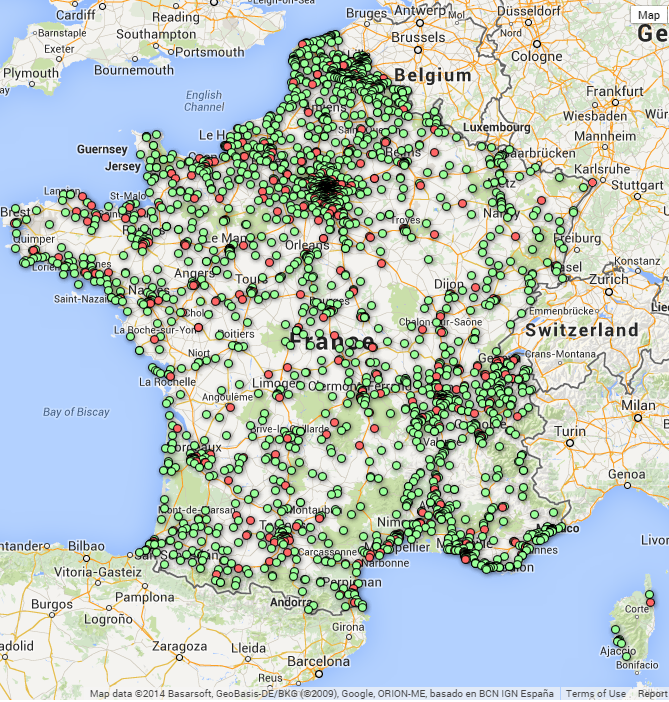
\includegraphics[width=16cm]{images/CARREFOUR.png}
\end{figure}

\begin{figure}[!h]
    \caption{CASINO}
	\centering
		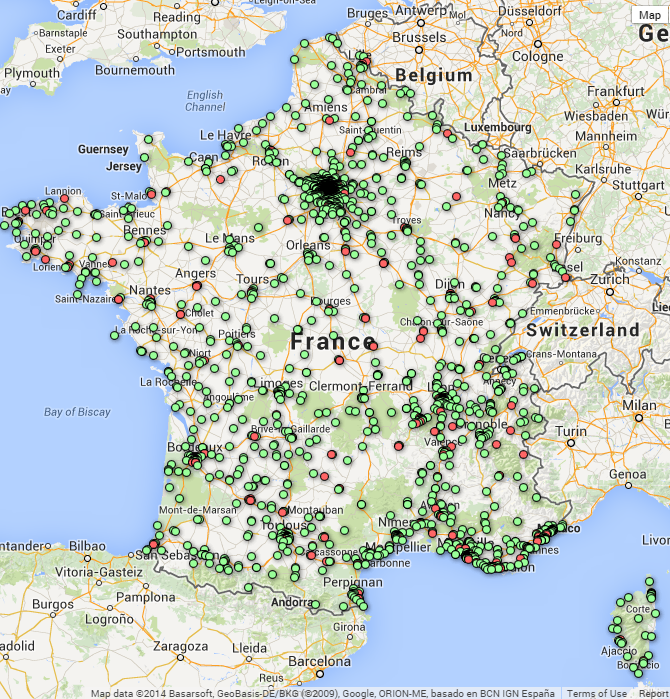
\includegraphics[width=16cm]{images/CASINO.png}
\end{figure}

\begin{figure}[!h]
    \caption{MOUSQUETAIRES}
	\centering
		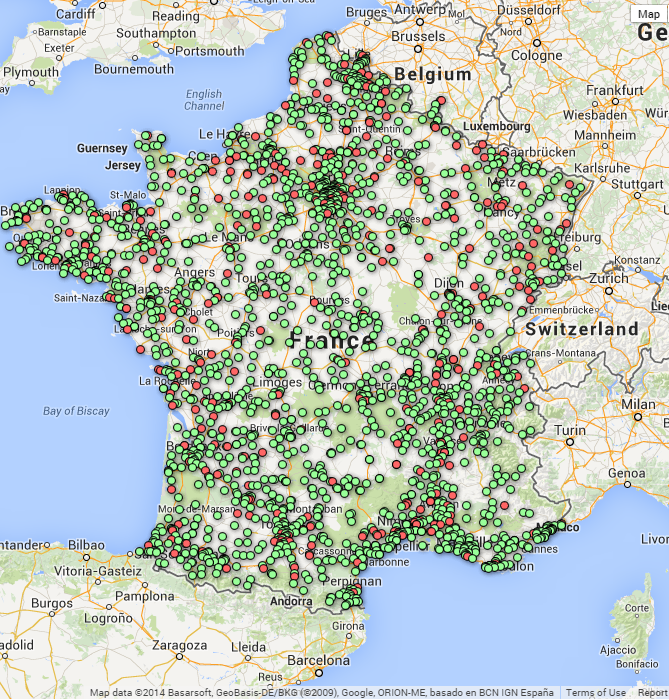
\includegraphics[width=16cm]{images/MOUSQUETAIRES.png}
\end{figure}

\begin{figure}[!h]
    \caption{LIDL}
	\centering
		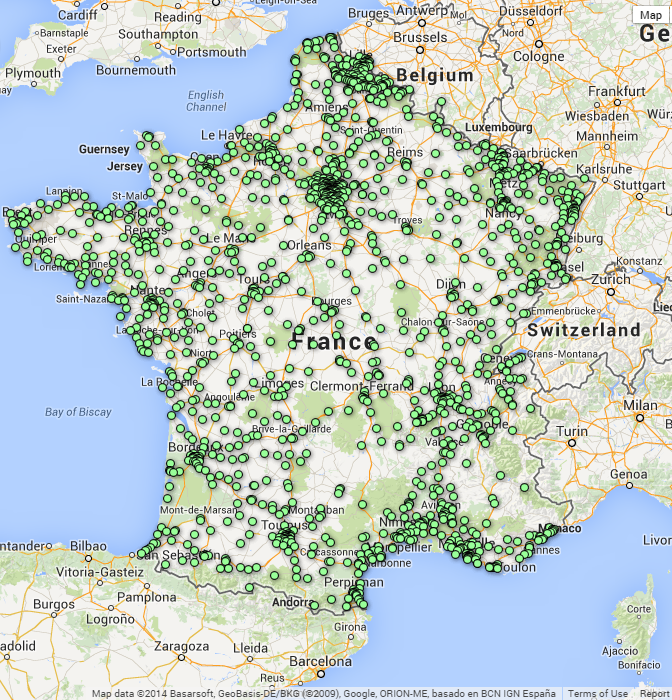
\includegraphics[width=16cm]{images/LIDL.png}
\end{figure}

\begin{figure}[!h]
    \caption{SYSTEME U}
	\centering
		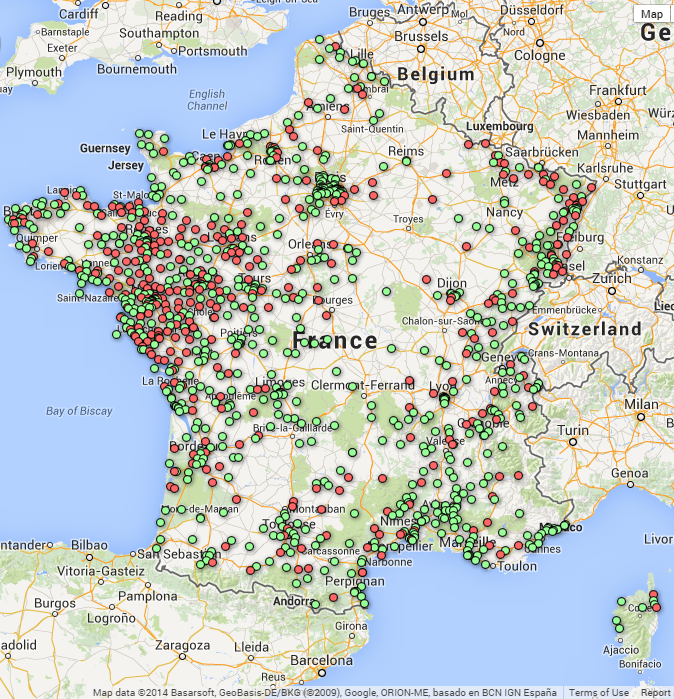
\includegraphics[width=16cm]{images/SYSTEME_U.png}
\end{figure}

\begin{figure}[!h]
    \caption{ALDI}
	\centering
		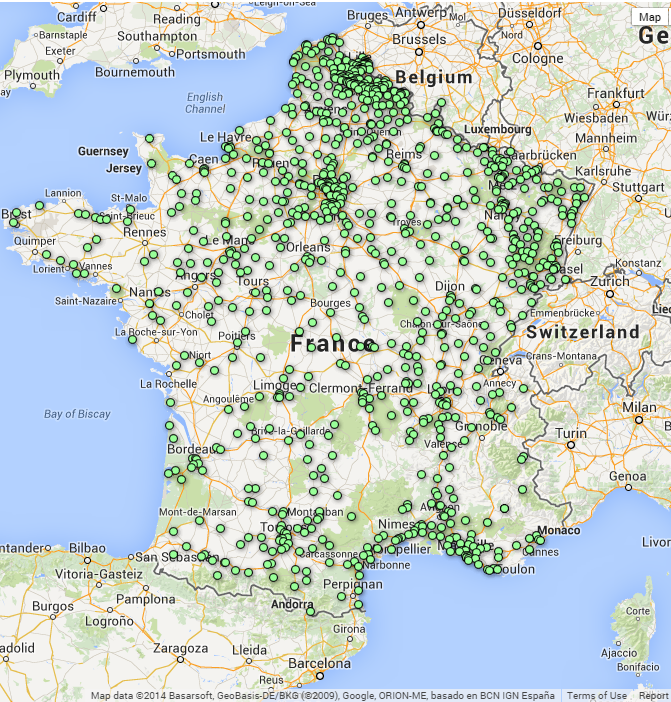
\includegraphics[width=16cm]{images/ALDI.png}
\end{figure}

\begin{figure}[!h]
    \caption{LECLERC}
	\centering
		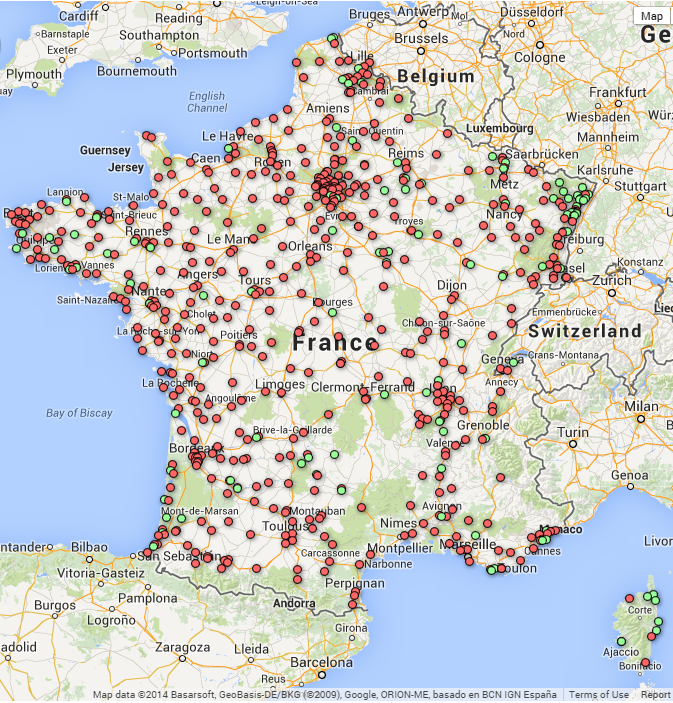
\includegraphics[width=16cm]{images/LECLERC.png}
\end{figure}

\begin{figure}[!h]
    \caption{AUCHAN}
	\centering
		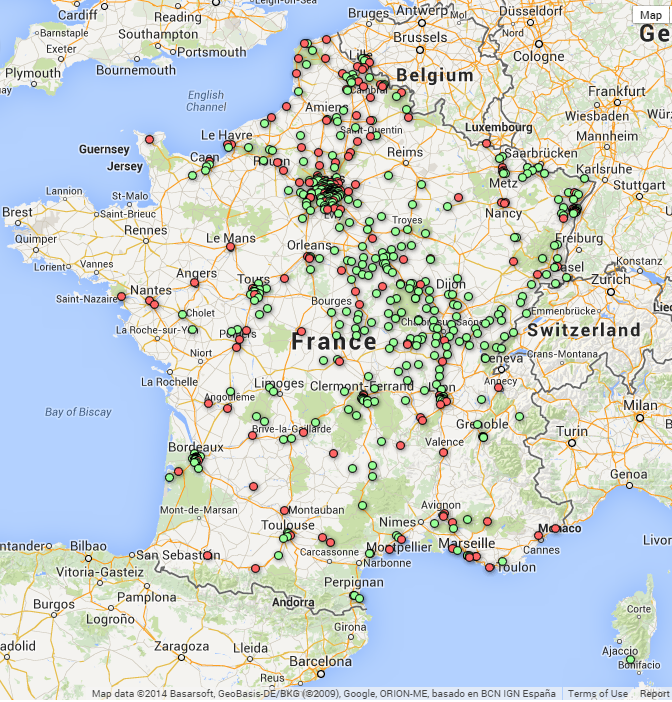
\includegraphics[width=16cm]{images/AUCHAN.png}
\end{figure}

\begin{figure}[!h]
    \caption{LOUIS DELHAIZE}
	\centering
		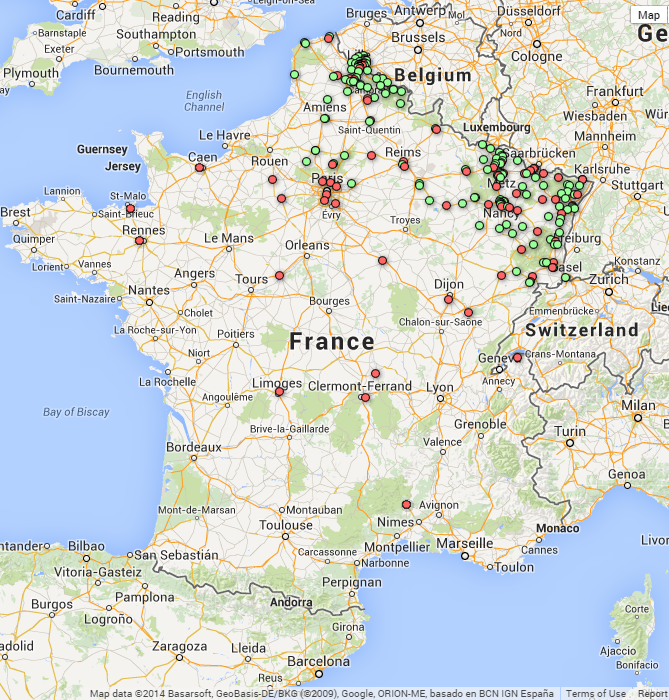
\includegraphics[width=16cm]{images/LOUIS_DELHAIZE.png}
\end{figure}

\begin{figure}[!h]
    \caption{DIAPAR}
	\centering
		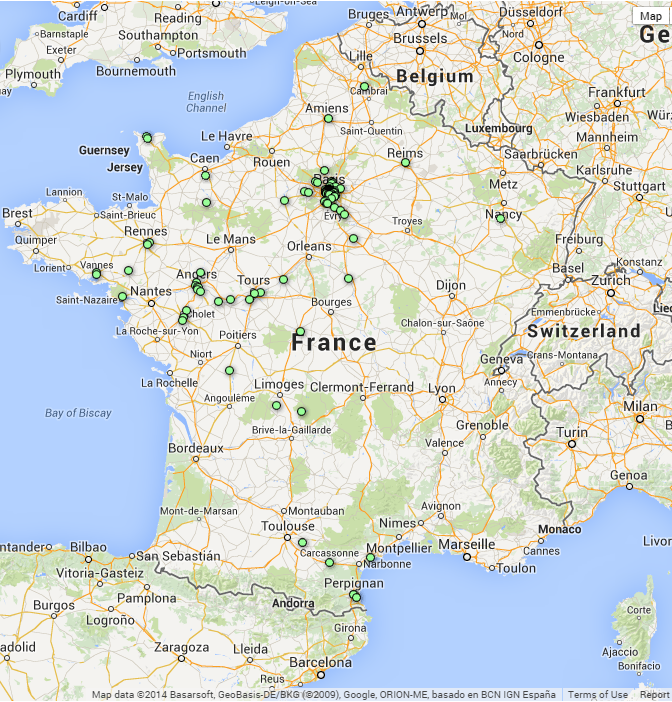
\includegraphics[width=16cm]{images/DIAPAR.png}
\end{figure}


\begin{figure}[!h]
    \caption{COLRUYT}
	\centering
		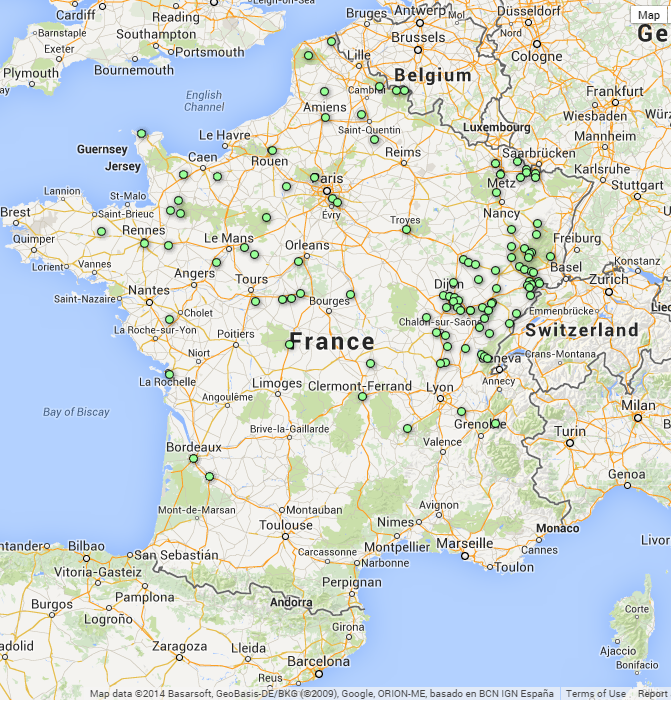
\includegraphics[width=16cm]{images/COLRUYT.png}
\end{figure}

\begin{figure}[!h]
    \caption{OTHER}
	\centering
		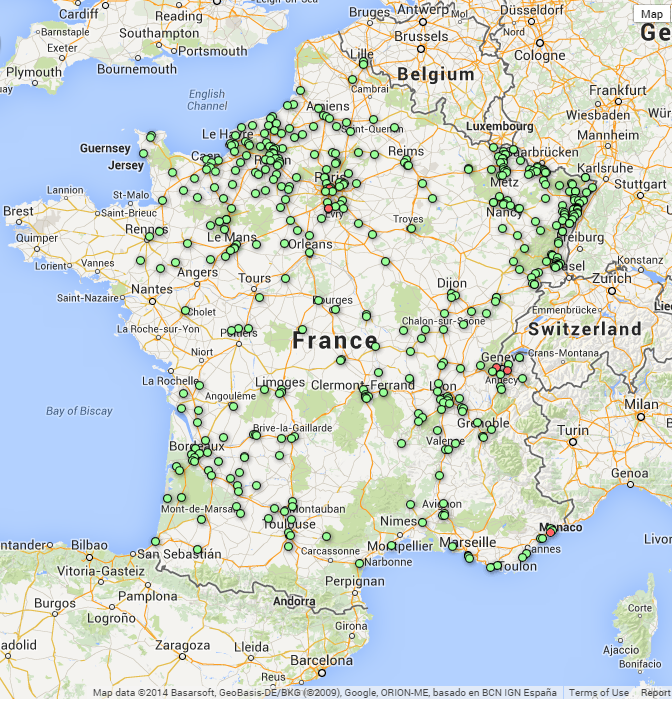
\includegraphics[width=16cm]{images/AUTRE.png}
\end{figure}

\end{document}
